\documentclass[12pt]{article}
\usepackage[utf8]{inputenc}
\usepackage[T2A]{fontenc}
\usepackage[russian]{babel}
\usepackage{amsmath, amssymb}
\usepackage{geometry}
\usepackage{graphicx}
\usepackage{titlesec} % Для настройки заголовков
\usepackage{enumitem} % Для настройки списков
\usepackage{fancyhdr} % Для колонтитулов
\usepackage{tabularx} % Для таблиц
\usepackage{lastpage} % Для номера последней страницы



% --- НАСТРОЙКА СТИЛЯ ---
\geometry{a4paper, left=25mm, right=15mm, top=20mm, bottom=20mm, headheight=15pt}
\setlength{\parindent}{0pt} % Убираем абзацный отступ
\setlist[enumerate]{topsep=5pt, itemsep=8pt, leftmargin=25pt} % Настройка списков
\titleformat{\section}{\large\bfseries\centering}{\thesection}{1em}{} % Стиль секций

% --- КОЛОНТИТУЛЫ (со 2-й страницы) ---
\pagestyle{fancy}
\fancyhf{}
\fancyhead[L]{
\includegraphics[height=1.1cm]{logo.png} \textbf{MathCore} | MOCK Test-1}
\fancyhead[R]{Abdunazarov M.X.}
\fancyfoot[C]{}
\renewcommand{\headrulewidth}{0.4pt}

\title{MOCK Test-1}
\author{Abdunazarov M.X.}
\date{}
\begin{document}

\maketitle
\begin{center}
  
\includegraphics[width=5cm]{logo.png}
\end{center}
\begin{enumerate}

\item Agar \( f(2x+1) + f(x+2) = x^2 - 5x + 3 \) bo'lsa, \( f'(3) \) ni toping.
\\ A) -1,5    
B) -1    
C) 0    
D) 1
\vspace{4cm}

\item \( \sqrt{y^2 + 1} = x y y' \) differensial tenglamani yeching.
\\ A) \( \sqrt{y^2 + 1} = \ln x + C \)    
B) \( \sqrt{y^2 + 1} = 2 \ln x + C \)    
C) \( \sqrt{y + 1} = \ln x^2 + C \)    
D) \( \sqrt{y^2 - 1} = \ln x + C \)
\vspace{4cm}

\item \( 5x - y + 7 = 0 \) va \( 2x - 3y + 1 = 0 \) to'g'ri chiziqlar orasidagi o'tmas burchakni toping.
\\ A) 45°    
B) 60°    
C) 120°    
D) 135°
\vspace{4cm}

\item To'g'ri uchburchak prizmada asos tomonlari 6, 8, 10 ga, yon qirrasi 15 ga teng. Asosning kichik balandligi va yon qirra orqali kesma o'tkazilgan. Kesma yuzini toping.
\\ A) 36    
B) 48    
C) 60    
D) 72
\vspace{4cm}

\item Agar \( f(2x+1) = x^2 + 6x + 12 \) bo'lsa, \( f'(5) \) ni toping.
\\ A) 2    
B) 5    
C) 2,5    
D) 5,5
\vspace{4cm}

\item Agar \( f(x) + f'(x) = x^3 + 2x^2 + 4x + 1 \) bo'lsa, \( f(x-1) \) funksiyasini toping.
\\ A) \( f(x-1) = x^3 - x^2 + 6x - 5 \)    
B) \( f(x-1) = x^4 + x^3 - 6x - 5 \)    
C) \( f(x-1) = x^4 - x^3 + 6x - 5 \)    
D) \( f(x-1) = x^3 - 4x^2 + 11x - 13 \)
\vspace{4cm}

\item Soat 12:40 da soat va minut milʼlari orasidagi burchakni toping.
\\ A) 240°    
B) 140°    
C) 160°    
D) 80°
\vspace{4cm}

\item Ketma-ket uchta toq sonning yig'indisi 12021 ga teng. Ularning eng kichigini toping.
\\ A) 2007    
B) 2003    
C) 4005    
D) 4013
\vspace{4cm}

\item \( 2^{2024} + 1 \) sonini 17 ga bo'lgandagi qoldiqni toping.
\\ A) 1    
B) 2    
C) 16    
D) 0
\vspace{4cm}

\item \( 10^{2721} + 5 \) sonini 17 ga bo'lgandagi qoldiqni toping.
\\ A) 16    
B) 15    
C) 10    
D) 14
\vspace{4cm}

\item 3 ga karrali bo'lgan ketma-ket ikkita m va n sonlar uchun EKUB(m;n) + EKUK(m;n) = 471. m + n ni toping.
\\ A) 36    
B) 39    
C) 75    
D) 81
\vspace{4cm}

\item Agar \( \int (f'(x) - 2x) dx = 2f(x) + x^3 - x^2 \) bo'lsa, \( f'(1) \) ni toping.
\\ A) 3    
B) -1    
C) 1    
D) -3
\vspace{4cm}

\item \( f(x) = \sin 2x \) funksiyaning \( M(0;1) \) nuqtadan o'tuvchi boshlang'ich funksiyasini toping.
\\ A) \( -\cos 2x + 2 \)    
B) \( -\frac{1}{2} \cos 2x + \frac{3}{2} \)    
C) \( \frac{1}{2} \cos 2x + \frac{1}{2} \)    
D) \( \cos 2x \)
\vspace{4cm}

\item \( x_1 \) va \( x_2 \) sonlar \( x^2 - (m + 4)x + 2m - 1 = 0 \) tenglamaning ildizlari. \( x_1^2 x_2 + x_1 x_2^2 \leq 0 \) tengsizlik nechta butun m qiymatlarida bajariladi?
\\ A) 2    
B) 3    
C) 4    
D) 5
\vspace{4cm}

\item Agar \( 4f(x) + f(2\pi - x) = 2x^3 + 8 \) bo'lsa, \( f'(\pi) \) ni toping.
\\ A) \( 6\pi^2 \)    
B) \( 3\pi^2 \)    
C) \( 2\pi^2 \)    
D) \( 4\pi^2 \)
\vspace{4cm}

\item Agar \( \int f(x)dx = x^3 + 3x^2 + mx + n \) va \( f(1) = 10 \) bo'lsa, \( F(3) - F(0) \) ni toping. (Bu yerda \( F(x) \) - \( f(x) \) funksiyaning boshlang'ich funksiyasi)
\\ A) 53    
B) 57    
C) 59    
D) aniqlab bo'lmaydi
\vspace{4cm}

\item 3 ta g'oz, 4 ta o'rdak va 2 ta tovuqdan har xil turdagi bittadan qush tanlab, nechta guruh tuzish mumkin?
\\ A) 10    
B) 12    
C) 18    
D) 24
\vspace{4cm}

\item Uchburchak piramida asosining tomonlari 25, 29 va 36 ga teng. Barcha yon qirralar asos tekisligi bilan bir xil burchak tashkil qiladi, balandligi 6 ga teng. Shu piramidaga ichki chizilgan konusning hajmini toping.
\\ A) 288\(\pi\)    
B) 244\(\pi\)    
C) 144\(\pi\)    
D) 128\(\pi\)
\vspace{4cm}

\item Tomonlari 5, 8, 12 ga teng va o'zaro perpendikulyar bo'lgan qirralarga ega uchburchak piramidaning hajmini toping.
\\ A) 120    
B) 100    
C) 80    
D) 60
\vspace{4cm}

\item Kvadrat funksiya \( y = ax^2 + bx + c \) grafigi berilgan. Grafikka asosan a, b, c ni solishtiring.
\begin{center}
    \centering
    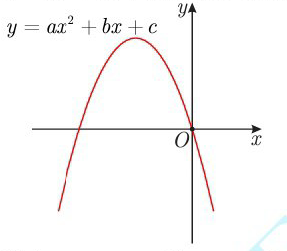
\includegraphics[width=0.5\linewidth]{6.png}
\end{center}
\\ A) \(b < a < c\)    
B) \(a < c < b\)    
C) \(b < x < a\)    
D) \(c < a < b\)
\vspace{4cm}

\item A truba bo'sh idishni 6 soatda, B truba bo'sh idishni 3 soatda to'ldiradi. C truba idishning \( \frac{2}{3} \) qismini 4 soatda bo'shatadi. Agar uchala truba bir vaqtda ishlasa, bo'sh idish necha soatda to'ladi?
\begin{center}
    \centering
    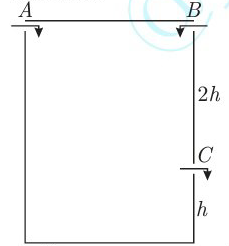
\includegraphics[width=0.5\linewidth]{7.png}
\end{center}
\\ A) \(\frac{8}{3}\)    
B) 2,5    
C) \(\frac{7}{5}\)    
D) \(\frac{9}{5}\)
\vspace{4cm}

\item \( y = x^2 + 1 \) va \( y = 2 \) egri chiziqlar bilan chegaralangan sohani Oy o'qi atrofida aylantirishdan hosil bo'lgan jismning hajmini toping.
\\ A) \(\frac{\pi}{2}\)    
B) \(\frac{2\pi}{3}\)    
C) \(\frac{3\pi}{2}\)    
D) \(\pi\)
\vspace{4cm}

\item \( y'(x + 1) = x y \) differensial tenglamani yeching.
\\ A) \( y = \frac{Ce^x}{x+1} \)    
B) \( y = \frac{Ce^x}{x-1} \)    
C) \( y = C(x+1)e^x \)    
D) \( y = C(x+1)e^{-x} \)
\vspace{4cm}

\item Kichik doiralarning radiusi \( r = 2 \) ga teng. Yashil rang bilan bo'yalgan sohaning yuzini toping.
\begin{center}
    \centering
    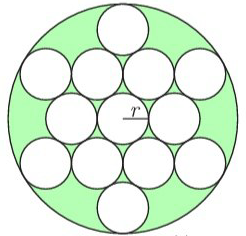
\includegraphics[width=0.5\linewidth]{8.png}
\end{center}
\\ A) \( 8\sqrt{3}\pi \)    
B) \( \frac{44}{\sqrt{3}}\pi \)    
C) \( \frac{52}{\sqrt{3}}\pi \)    
D) \( 16\sqrt{3}\pi \)
\vspace{4cm}

\item Birinchi qotishmada metallarning nisbati 2:3, ikkinchi qotishmada esa 3:4. Metallar nisbati 11:15 bo'lgan qotishma olish uchun bu qotishmalarni qanday nisbatda olish kerak?
\\ A) birinchi qotishma 5 qism, ikkinchi qotishma 21 qism    
B) birinchi qotishma 6 qism, ikkinchi qotishma 20 qism    
C) birinchi qotishma 7 qism, ikkinchi qotishma 19 qism    
D) birinchi qotishma 8 qism, ikkinchi qotishma 18 qism
\vspace{4cm}

\item Agar ABCD kvadrat bo'lsa (BE = EC, AK = KB, AB = 10), EFG uchburchak yuzini toping.
\begin{center}
    \centering
    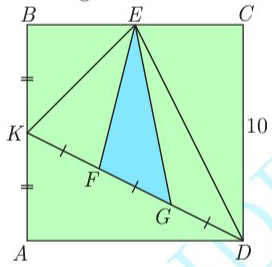
\includegraphics[width=0.5\linewidth]{9.png}
\end{center}
\\ A) 14    
B) 12,5    
C) 12    
D) \( 8\frac{1}{3} \)
\vspace{4cm}

\item Agar \( P_{EDC} = 16 \) va \( AB = 15 \) bo'lsa, \( P_{ABC} \) ni toping.
\begin{center}
    \centering
    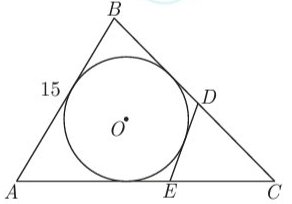
\includegraphics[width=0.5\linewidth]{11.png}
\end{center}
\\ A) 30    
B) 40    
C) 46    
D) 47
\vspace{4cm}

\item To'rtta son berilgan. Dastlabki uchtasi geometrik progressiya, oxirgi uchtasi arifmetik progressiya tashkil qiladi. Chekki sonlar yig'indisi 21, o'rta sonlar yig'indisi 18 ga teng. Barcha to'rtta sonning ko'paytmasini toping.
\\ A) 3636    
B) 3838    
C) 3888    
D) 3996
\vspace{4cm}

\item Rasmdagi maʼlumotlardan foydalanib, x ni toping.
\begin{center}
    \centering
    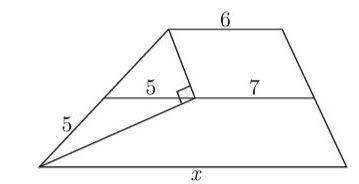
\includegraphics[width=0.5\linewidth]{12.png}
\end{center}
\\ A) 15    
B) 16    
C) 17    
D) 18
\vspace{4cm}

\item Talabalarning 75\% A tilini, 65\% B tilini biladi. Ikkala tilni ham biladigan talabalar soni hech qaysi tilni bilmaydigan talabalar sonidan 3 marta ko'p. Ikkala tilni ham biladigan talabalar foizini toping.
\\ A) 60\%    
B) 45\%    
C) 50\%    
D) 55\%
\vspace{4cm}

\item Agar \( \int_{-1}^{2} x \cdot f'(x) dx = 10 \) bo'lsa, \( \int_{-1}^{2} f(x) dx \) ni toping.
\begin{center}
    \centering
    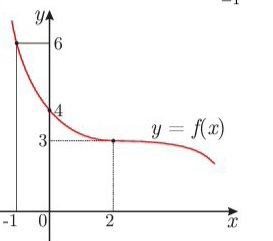
\includegraphics[width=0.5\linewidth]{13.png}
\end{center}
\\ A) 0    
B) 2    
C) 4    
D) -4
\vspace{4cm}

\item \( y = k e^{\frac{x}{2}} \), \( x = 2 \), \( x = 0 \) va \( y = 0 \) chiziqlar bilan chegaralangan sohaning yuzi shu sohani Ox o'qi atrofida aylantirishdan hosil bo'lgan jismning hajmiga teng bo'ladigan k qiymatini toping.
\\ A) \(\frac{2}{\pi(e-1)}\)    
B) \(\frac{2e}{\pi}\)    
C) \(\frac{2}{\pi(e+1)}\)    
D) \(\frac{2}{e\pi}\)
\vspace{4cm}

\item \( y = \sqrt{x} \) va \( y = \frac{x}{2} \) chiziqlar bilan chegaralangan sohani Oy o'qi atrofida aylantirishdan hosil bo'lgan jismning hajmini toping.
\\ A) \(\frac{64}{15}\pi\)    
B) 9,6\(\pi\)    
C) 9\(\pi\)    
D) \(\frac{15}{2}\pi\)
\vspace{4cm}

\item Birinchi holatda bola 2 N kuch bilan yukni ko'taradi, bunda kuchning balandlik bo'yicha hosilasi \( \frac{dF}{dh} = \frac{1}{\sqrt{h}} + 3 + \frac{1}{h+1} \) berilgan. Ikkinchi holatda u qancha kuch (N da) sarflaydi?
\begin{center}
    \centering
    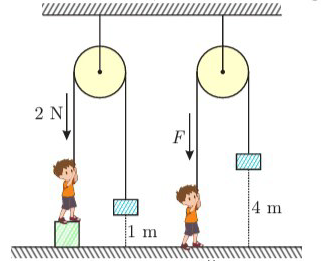
\includegraphics[width=0.5\linewidth]{14.png}
\end{center}
\\ A) 13    
B) \( 13 - \ln \frac{5}{2} \)    
C) \( 13 + \ln \frac{5}{2} \)    
D) 11,5
\vspace{4cm}

\item Asosi tomonlari 25, 29, 36 ga teng va balandligi 6 ga teng uchburchak piramidaga ichki chizilgan sfera radiusini toping.
\\ A) \(\frac{10}{3}\)    
B) \(\frac{7}{3}\)    
C) \(\frac{7}{2}\)    
D) \(\frac{8}{3}\)
\vspace{4cm}

\end{enumerate}

\end{document}